\documentclass[]{article}
\usepackage{lmodern}
\usepackage{amssymb,amsmath}
\usepackage{ifxetex,ifluatex}
\usepackage{fixltx2e} % provides \textsubscript
\ifnum 0\ifxetex 1\fi\ifluatex 1\fi=0 % if pdftex
  \usepackage[T1]{fontenc}
  \usepackage[utf8]{inputenc}
\else % if luatex or xelatex
  \ifxetex
    \usepackage{mathspec}
  \else
    \usepackage{fontspec}
  \fi
  \defaultfontfeatures{Ligatures=TeX,Scale=MatchLowercase}
\fi
% use upquote if available, for straight quotes in verbatim environments
\IfFileExists{upquote.sty}{\usepackage{upquote}}{}
% use microtype if available
\IfFileExists{microtype.sty}{%
\usepackage{microtype}
\UseMicrotypeSet[protrusion]{basicmath} % disable protrusion for tt fonts
}{}
\usepackage[margin=1in]{geometry}
\usepackage{hyperref}
\hypersetup{unicode=true,
            pdftitle={Singular Value Decomposition for Federated Data},
            pdfborder={0 0 0},
            breaklinks=true}
\urlstyle{same}  % don't use monospace font for urls
\usepackage{color}
\usepackage{fancyvrb}
\newcommand{\VerbBar}{|}
\newcommand{\VERB}{\Verb[commandchars=\\\{\}]}
\DefineVerbatimEnvironment{Highlighting}{Verbatim}{commandchars=\\\{\}}
% Add ',fontsize=\small' for more characters per line
\usepackage{framed}
\definecolor{shadecolor}{RGB}{248,248,248}
\newenvironment{Shaded}{\begin{snugshade}}{\end{snugshade}}
\newcommand{\KeywordTok}[1]{\textcolor[rgb]{0.13,0.29,0.53}{\textbf{#1}}}
\newcommand{\DataTypeTok}[1]{\textcolor[rgb]{0.13,0.29,0.53}{#1}}
\newcommand{\DecValTok}[1]{\textcolor[rgb]{0.00,0.00,0.81}{#1}}
\newcommand{\BaseNTok}[1]{\textcolor[rgb]{0.00,0.00,0.81}{#1}}
\newcommand{\FloatTok}[1]{\textcolor[rgb]{0.00,0.00,0.81}{#1}}
\newcommand{\ConstantTok}[1]{\textcolor[rgb]{0.00,0.00,0.00}{#1}}
\newcommand{\CharTok}[1]{\textcolor[rgb]{0.31,0.60,0.02}{#1}}
\newcommand{\SpecialCharTok}[1]{\textcolor[rgb]{0.00,0.00,0.00}{#1}}
\newcommand{\StringTok}[1]{\textcolor[rgb]{0.31,0.60,0.02}{#1}}
\newcommand{\VerbatimStringTok}[1]{\textcolor[rgb]{0.31,0.60,0.02}{#1}}
\newcommand{\SpecialStringTok}[1]{\textcolor[rgb]{0.31,0.60,0.02}{#1}}
\newcommand{\ImportTok}[1]{#1}
\newcommand{\CommentTok}[1]{\textcolor[rgb]{0.56,0.35,0.01}{\textit{#1}}}
\newcommand{\DocumentationTok}[1]{\textcolor[rgb]{0.56,0.35,0.01}{\textbf{\textit{#1}}}}
\newcommand{\AnnotationTok}[1]{\textcolor[rgb]{0.56,0.35,0.01}{\textbf{\textit{#1}}}}
\newcommand{\CommentVarTok}[1]{\textcolor[rgb]{0.56,0.35,0.01}{\textbf{\textit{#1}}}}
\newcommand{\OtherTok}[1]{\textcolor[rgb]{0.56,0.35,0.01}{#1}}
\newcommand{\FunctionTok}[1]{\textcolor[rgb]{0.00,0.00,0.00}{#1}}
\newcommand{\VariableTok}[1]{\textcolor[rgb]{0.00,0.00,0.00}{#1}}
\newcommand{\ControlFlowTok}[1]{\textcolor[rgb]{0.13,0.29,0.53}{\textbf{#1}}}
\newcommand{\OperatorTok}[1]{\textcolor[rgb]{0.81,0.36,0.00}{\textbf{#1}}}
\newcommand{\BuiltInTok}[1]{#1}
\newcommand{\ExtensionTok}[1]{#1}
\newcommand{\PreprocessorTok}[1]{\textcolor[rgb]{0.56,0.35,0.01}{\textit{#1}}}
\newcommand{\AttributeTok}[1]{\textcolor[rgb]{0.77,0.63,0.00}{#1}}
\newcommand{\RegionMarkerTok}[1]{#1}
\newcommand{\InformationTok}[1]{\textcolor[rgb]{0.56,0.35,0.01}{\textbf{\textit{#1}}}}
\newcommand{\WarningTok}[1]{\textcolor[rgb]{0.56,0.35,0.01}{\textbf{\textit{#1}}}}
\newcommand{\AlertTok}[1]{\textcolor[rgb]{0.94,0.16,0.16}{#1}}
\newcommand{\ErrorTok}[1]{\textcolor[rgb]{0.64,0.00,0.00}{\textbf{#1}}}
\newcommand{\NormalTok}[1]{#1}
\usepackage{graphicx,grffile}
\makeatletter
\def\maxwidth{\ifdim\Gin@nat@width>\linewidth\linewidth\else\Gin@nat@width\fi}
\def\maxheight{\ifdim\Gin@nat@height>\textheight\textheight\else\Gin@nat@height\fi}
\makeatother
% Scale images if necessary, so that they will not overflow the page
% margins by default, and it is still possible to overwrite the defaults
% using explicit options in \includegraphics[width, height, ...]{}
\setkeys{Gin}{width=\maxwidth,height=\maxheight,keepaspectratio}
\IfFileExists{parskip.sty}{%
\usepackage{parskip}
}{% else
\setlength{\parindent}{0pt}
\setlength{\parskip}{6pt plus 2pt minus 1pt}
}
\setlength{\emergencystretch}{3em}  % prevent overfull lines
\providecommand{\tightlist}{%
  \setlength{\itemsep}{0pt}\setlength{\parskip}{0pt}}
\setcounter{secnumdepth}{0}
% Redefines (sub)paragraphs to behave more like sections
\ifx\paragraph\undefined\else
\let\oldparagraph\paragraph
\renewcommand{\paragraph}[1]{\oldparagraph{#1}\mbox{}}
\fi
\ifx\subparagraph\undefined\else
\let\oldsubparagraph\subparagraph
\renewcommand{\subparagraph}[1]{\oldsubparagraph{#1}\mbox{}}
\fi

%%% Use protect on footnotes to avoid problems with footnotes in titles
\let\rmarkdownfootnote\footnote%
\def\footnote{\protect\rmarkdownfootnote}

%%% Change title format to be more compact
\usepackage{titling}

% Create subtitle command for use in maketitle
\providecommand{\subtitle}[1]{
  \posttitle{
    \begin{center}\large#1\end{center}
    }
}

\setlength{\droptitle}{-2em}

  \title{Singular Value Decomposition for Federated Data}
    \pretitle{\vspace{\droptitle}\centering\huge}
  \posttitle{\par}
    \author{true \\ true}
    \preauthor{\centering\large\emph}
  \postauthor{\par}
      \predate{\centering\large\emph}
  \postdate{\par}
    \date{2019-06-20}


\begin{document}
\maketitle

\section{Purpose of this package}\label{purpose-of-this-package}

Analyzing data across hospitals and institutions without the data
leaving the hospitals and adding institutions to a trusted network is an
important part of privacy preserving data analysis. In order to assure
all of this we can use DataSHIELD, an open source solution that let
researchers analyze microdata without physically sharing this data with
them. It allows a standardized, monitored, indirect and secure access to
data.

The aim of this package is to provide functions that compute the
Singular Value Decomposition of large matrices and perform a Principal
Component Analysis when we do not have access to the whole dataset, as
in DataSHIELD \footnote{http://www.datashield.ac.uk/}. At the same time,
we are interested in the high computational cost that computing a SVD
has, so we present some functions that calculate SVD's and PCA's in a
more efficient way. The functions in this package can be classified in
two different blocks: Jacobi algorithm and Block algorithm. The first
group contains functions that perform a SVD using functions that apply
the two sided Jacobi algorithm. This is an iterative algorithm that is
also parallelizable and could perform well with large datasets and multi
cores processors. However, it cannot be applied to DataSHIELD. The
second group uses an incremental algorithm that we call Block method and
consists of partitioning the matrix under study in submatrices in order
to reduce their dimension and compute the SVD faster. This is applicable
to DataSHIELD.

The Block method allows us to compute a PCA of different datasets
without being able to join them. However, to do so we need that each
dataset contains the same variables and a greater number of individuals
than variables. This usually happens in most of the datasets.
Nevertheless this is not the case for omic data. In this case, Block
functions will not be useful for DataSHIELD but they will be good to
perform efficient calculations in large datasets.

\section{Getting started}\label{getting-started}

First, you can install \texttt{svdParallel} from Github by typing

\begin{Shaded}
\begin{Highlighting}[]
\NormalTok{devtools}\OperatorTok{::}\KeywordTok{install_github}\NormalTok{(}\StringTok{"isglobal-brge/svdParallel"}\NormalTok{)}
\end{Highlighting}
\end{Shaded}

Then, you can load the required packages to reproduce this document.

\begin{Shaded}
\begin{Highlighting}[]
\KeywordTok{library}\NormalTok{(svdParallel)}
\KeywordTok{library}\NormalTok{(FactoMineR)}
\KeywordTok{library}\NormalTok{(irlba)}
\KeywordTok{library}\NormalTok{(doParallel)}
\KeywordTok{library}\NormalTok{(devtools)}
\KeywordTok{library}\NormalTok{(Biobase)}
\KeywordTok{library}\NormalTok{(MultiDataSet)}
\KeywordTok{library}\NormalTok{(made4)}
\KeywordTok{library}\NormalTok{(brgedata)}
\KeywordTok{library}\NormalTok{(parallel)}
\KeywordTok{library}\NormalTok{(SummarizedExperiment)}
\end{Highlighting}
\end{Shaded}

In the following sections of this document we will present some examples
in order to make clear how the different functions work. To do so we
will use three datasets: \texttt{iris}, \texttt{breast} and
\texttt{breastTCGA}. The \texttt{iris} dataset is an R dataset and the
other two, \texttt{breast} and \texttt{breastTCGA}, are saved in the
data folder of this project, so you can access and manipulate all of
them.

\section{Computing a PCA using Jacobi
algorithm}\label{computing-a-pca-using-jacobi-algorithm}

In this case we will use the \texttt{iris} dataset. We can see the head
of this dataset as follows

\begin{Shaded}
\begin{Highlighting}[]
\KeywordTok{head}\NormalTok{(iris)}
\NormalTok{  Sepal.Length Sepal.Width Petal.Length Petal.Width Species}
\DecValTok{1}          \FloatTok{5.1}         \FloatTok{3.5}          \FloatTok{1.4}         \FloatTok{0.2}\NormalTok{  setosa}
\DecValTok{2}          \FloatTok{4.9}         \FloatTok{3.0}          \FloatTok{1.4}         \FloatTok{0.2}\NormalTok{  setosa}
\DecValTok{3}          \FloatTok{4.7}         \FloatTok{3.2}          \FloatTok{1.3}         \FloatTok{0.2}\NormalTok{  setosa}
\DecValTok{4}          \FloatTok{4.6}         \FloatTok{3.1}          \FloatTok{1.5}         \FloatTok{0.2}\NormalTok{  setosa}
\DecValTok{5}          \FloatTok{5.0}         \FloatTok{3.6}          \FloatTok{1.4}         \FloatTok{0.2}\NormalTok{  setosa}
\DecValTok{6}          \FloatTok{5.4}         \FloatTok{3.9}          \FloatTok{1.7}         \FloatTok{0.4}\NormalTok{  setosa}
\end{Highlighting}
\end{Shaded}

We need to remove the last column because it is a categorical variable
that we are not able to use in a PCA. We will use it later to analyze
the results.

\begin{Shaded}
\begin{Highlighting}[]
\KeywordTok{head}\NormalTok{(iris}\OperatorTok{$}\NormalTok{Species)}
\NormalTok{[}\DecValTok{1}\NormalTok{] setosa setosa setosa setosa setosa setosa}
\NormalTok{Levels}\OperatorTok{:}\StringTok{ }\NormalTok{setosa versicolor virginica}

\NormalTok{i <-}\StringTok{ }\NormalTok{iris[,}\OperatorTok{-}\DecValTok{5}\NormalTok{]}
\end{Highlighting}
\end{Shaded}

The function that performs a PCA is \texttt{getPCA} and we have to set
the method that we want to use to compute this PCA. The default method
is the Block method, so if we want to compute the PCA using the Jacobi
method we need to specify it. After computing a PCA with \texttt{getPCA}
we can use function \texttt{print} to see the main values obtained with
the PCA, the variance of each component and the percentage of variance
explained.

\begin{Shaded}
\begin{Highlighting}[]
\NormalTok{gJ <-}\StringTok{ }\KeywordTok{getPCA}\NormalTok{(i,}\DataTypeTok{method=}\StringTok{"Jacobi"}\NormalTok{)}
\KeywordTok{print}\NormalTok{(gJ)}
\OperatorTok{**}\NormalTok{Results }\ControlFlowTok{for}\NormalTok{ the Principal Component Analysis using method }\StringTok{'Jacobi'} \OperatorTok{**}

\NormalTok{Variance of the components}
\NormalTok{          PC1       PC2       PC3        PC4}
\NormalTok{[}\DecValTok{1}\NormalTok{,] }\FloatTok{2.918498} \FloatTok{0.9140305} \FloatTok{0.1467569} \FloatTok{0.02071484}

\NormalTok{Percentatge of variance explained }\ControlFlowTok{for}\NormalTok{ each component}
\NormalTok{          PC1      PC2      PC3       PC4}
\NormalTok{[}\DecValTok{1}\NormalTok{,] }\FloatTok{72.96245} \FloatTok{22.85076} \FloatTok{3.668922} \FloatTok{0.5178709}
\end{Highlighting}
\end{Shaded}

Now, we can plot the results using function \texttt{plot}. We need to
specify what type of plot we want, individuals or variables. Moreover,
if we do not specify anything more the plot will be made in the first
two principal components.

\begin{Shaded}
\begin{Highlighting}[]
\KeywordTok{par}\NormalTok{(}\DataTypeTok{mfrow=}\KeywordTok{c}\NormalTok{(}\DecValTok{1}\NormalTok{,}\DecValTok{2}\NormalTok{))}
\KeywordTok{plot}\NormalTok{(gJ, }\DataTypeTok{type=}\StringTok{"variables"}\NormalTok{)}
\KeywordTok{plot}\NormalTok{(gJ, }\DataTypeTok{type=}\StringTok{"individuals"}\NormalTok{)}
\end{Highlighting}
\end{Shaded}

\begin{figure}

{\centering \includegraphics{svdParallel_files/figure-latex/unnamed-chunk-1-1} 

}

\caption{Variables and individuals projections from getPCA function using Jacobi method. Left plot shows the variables in to the two first principal components, while right plot corresponds to the individuals.}\label{fig:unnamed-chunk-1}
\end{figure}

If we want the plots in other components we can do it by adding
\texttt{comps=c(i,j)}, where i and j are the new components.

\begin{Shaded}
\begin{Highlighting}[]
\KeywordTok{par}\NormalTok{(}\DataTypeTok{mfrow=}\KeywordTok{c}\NormalTok{(}\DecValTok{1}\NormalTok{,}\DecValTok{2}\NormalTok{))}
\KeywordTok{plot}\NormalTok{(gJ, }\DataTypeTok{type=}\StringTok{"variables"}\NormalTok{, }\DataTypeTok{comps=}\KeywordTok{c}\NormalTok{(}\DecValTok{1}\NormalTok{,}\DecValTok{3}\NormalTok{))}
\KeywordTok{plot}\NormalTok{(gJ, }\DataTypeTok{type=}\StringTok{"individuals"}\NormalTok{, }\DataTypeTok{comps=}\KeywordTok{c}\NormalTok{(}\DecValTok{1}\NormalTok{,}\DecValTok{3}\NormalTok{))}
\end{Highlighting}
\end{Shaded}

\begin{figure}

{\centering \includegraphics{svdParallel_files/figure-latex/unnamed-chunk-2-1} 

}

\caption{Variables and individuals projections from getPCA function using Jacobi method. Left plot shows the variables into the first and third first principal components, while right plot corresponds to the individuals.}\label{fig:unnamed-chunk-2}
\end{figure}

The \texttt{getPCA} function returns a list of different variables that
we can use to perform a deeper analysis of the data. This variables are
the coordinates of the variables, the Y matrix containing the
coordinates of the individuals, the variance and percentage of variance
explained by each component, the V matrix of the SVD performed and the
method used.

In order to access to this variables we can do

\begin{Shaded}
\begin{Highlighting}[]
\NormalTok{gJ}\OperatorTok{$}\NormalTok{varcoord}
\NormalTok{                    PC1        PC2         PC3         PC4}
\NormalTok{Sepal.Length  }\FloatTok{0.8901688} \FloatTok{0.36082989}  \FloatTok{0.27565767} \OperatorTok{-}\FloatTok{0.03760602}
\NormalTok{Sepal.Width  }\OperatorTok{-}\FloatTok{0.4601427} \FloatTok{0.88271627} \OperatorTok{-}\FloatTok{0.09361987}  \FloatTok{0.01777631}
\NormalTok{Petal.Length  }\FloatTok{0.9915552} \FloatTok{0.02341519} \OperatorTok{-}\FloatTok{0.05444699}  \FloatTok{0.11534978}
\NormalTok{Petal.Width   }\FloatTok{0.9649790} \FloatTok{0.06399985} \OperatorTok{-}\FloatTok{0.24298265} \OperatorTok{-}\FloatTok{0.07535950}
\end{Highlighting}
\end{Shaded}

For instance, we can use the Y matrix with the coordinates of the
individuals to represent them according to the species they belong:

\begin{Shaded}
\begin{Highlighting}[]
\NormalTok{setosa <-}\StringTok{ }\NormalTok{iris}\OperatorTok{$}\NormalTok{Species }\OperatorTok{==}\StringTok{ "setosa"}  
\NormalTok{versicolor <-}\StringTok{ }\NormalTok{iris}\OperatorTok{$}\NormalTok{Species }\OperatorTok{==}\StringTok{ "versicolor"}
\NormalTok{virginica <-}\StringTok{ }\NormalTok{iris}\OperatorTok{$}\NormalTok{Species }\OperatorTok{==}\StringTok{ "virginica"}
\KeywordTok{plot}\NormalTok{(gJ}\OperatorTok{$}\NormalTok{Y[setosa,}\KeywordTok{c}\NormalTok{(}\DecValTok{1}\NormalTok{,}\DecValTok{2}\NormalTok{)], }\DataTypeTok{main=}\StringTok{"Individuals"}\NormalTok{,}
     \DataTypeTok{type=}\StringTok{"p"}\NormalTok{, }\DataTypeTok{col=}\StringTok{"blue"}\NormalTok{,}\DataTypeTok{xlab=}\StringTok{"PC1 (72.96%)"}\NormalTok{, }
     \DataTypeTok{ylab=}\StringTok{"PC2 (22.85%)"}\NormalTok{, }\DataTypeTok{xlim=}\KeywordTok{c}\NormalTok{(}\OperatorTok{-}\DecValTok{4}\NormalTok{,}\FloatTok{5.5}\NormalTok{))}
\KeywordTok{points}\NormalTok{(gJ}\OperatorTok{$}\NormalTok{Y[versicolor,}\KeywordTok{c}\NormalTok{(}\DecValTok{1}\NormalTok{,}\DecValTok{2}\NormalTok{)], }\DataTypeTok{col=}\StringTok{"red"}\NormalTok{)}
\KeywordTok{points}\NormalTok{(gJ}\OperatorTok{$}\NormalTok{Y[virginica,}\KeywordTok{c}\NormalTok{(}\DecValTok{1}\NormalTok{,}\DecValTok{2}\NormalTok{)], }\DataTypeTok{col=}\StringTok{"green"}\NormalTok{)}
\KeywordTok{legend}\NormalTok{(}\StringTok{"bottomright"}\NormalTok{, }\DataTypeTok{legend =} \KeywordTok{c}\NormalTok{(}\StringTok{"Setosa"}\NormalTok{, }\StringTok{"Versicolor"}\NormalTok{, }\StringTok{"Virginica"}\NormalTok{), }\DataTypeTok{col=}\KeywordTok{c}\NormalTok{(}\StringTok{"blue"}\NormalTok{, }\StringTok{"red"}\NormalTok{, }\StringTok{"green"}\NormalTok{), }\DataTypeTok{pch=}\DecValTok{1}\NormalTok{, }\DataTypeTok{cex=}\FloatTok{0.75}\NormalTok{)}
\end{Highlighting}
\end{Shaded}

\begin{figure}

{\centering \includegraphics{svdParallel_files/figure-latex/iris7-1} 

}

\caption{Principal components of iris dataset. The plot shows the samples according to the species they belong to.}\label{fig:iris7}
\end{figure}

As we can see, the individuals are classified according to the species.

we can perform the same calculations using \texttt{JacobiR} method. This
method is not parallelizable and it is faster than \texttt{Jacobi}. We
would recommend using \texttt{JacobiR} when we do not deal with big
matrices and we do not need to parallelize. However, in small matrices
the difference is not significant.

The functions that contain the Jacobi algorithm are \texttt{Jacobi},
\texttt{JacobiR} and \texttt{parJacobi} and they compute the eigenvalues
and eigenvectores of a real symmetric matrix using the two-sided Jacobi
algorithm. Functions \texttt{svdJacobi} and \texttt{svdJacobiR} compute
a SVD of a real rectangular matrix and returns the left and right
singular vectors and the singular values.

\begin{Shaded}
\begin{Highlighting}[]
\NormalTok{svdJ <-}\StringTok{ }\KeywordTok{svdJacobi}\NormalTok{(i)}
\NormalTok{svdJ}\OperatorTok{$}\NormalTok{d}
\NormalTok{Sepal.Length  Sepal.Width Petal.Length  Petal.Width }
   \FloatTok{95.959914}    \FloatTok{17.761034}     \FloatTok{3.460931}     \FloatTok{1.884826} 
\end{Highlighting}
\end{Shaded}

We have obtained the singular values of the iris dataset.

As these functions use an iterative method we need to set a tolerance.
The value set by default is the tolerance of the machine, but it can be
changed setting the \texttt{tol} parameter.

\section{Computing a PCA using Block method for
DataSHIELD.}\label{computing-a-pca-using-block-method-for-datashield.}

In this case we will also use \texttt{getPCA} function but we will
specify a different method. If we want to simulate that we are in a
DataSHIELD experiment and we cannot join the different datasets we can
use a list containing the datasets. To do so, we will use
\texttt{breast} dataset. We need to remove the categorical variables to
be able to work with the numerical ones.

\begin{Shaded}
\begin{Highlighting}[]
\NormalTok{breast[}\DecValTok{1}\OperatorTok{:}\DecValTok{5}\NormalTok{,}\DecValTok{1}\OperatorTok{:}\DecValTok{3}\NormalTok{]}
\NormalTok{        id diagnosis radius_mean}
\DecValTok{1}   \DecValTok{842302}\NormalTok{         M       }\FloatTok{17.99}
\DecValTok{2}   \DecValTok{842517}\NormalTok{         M       }\FloatTok{20.57}
\DecValTok{3} \DecValTok{84300903}\NormalTok{         M       }\FloatTok{19.69}
\DecValTok{4} \DecValTok{84348301}\NormalTok{         M       }\FloatTok{11.42}
\DecValTok{5} \DecValTok{84358402}\NormalTok{         M       }\FloatTok{20.29}
\NormalTok{num_breast <-}\StringTok{ }\NormalTok{breast[,}\DecValTok{3}\OperatorTok{:}\DecValTok{32}\NormalTok{]}
\KeywordTok{dim}\NormalTok{(num_breast)}
\NormalTok{[}\DecValTok{1}\NormalTok{] }\DecValTok{569}  \DecValTok{30}
\end{Highlighting}
\end{Shaded}

As we can see, the dimension of the dataset is 569 x 29. We can create
three datasets taking the first 200 individuals, the individuals in rows
between 201 and 400 and the last individuals from 401 to 569. These
datasets have the same variables and have more individuals than
variables. We can use the Block method to compute the SVD. This method
computes a SVD of each of the subsets and then joins the results to
compute a SVD again. In the following figure we can see a flowchart of
the procedure:

\begin{figure}

{\centering 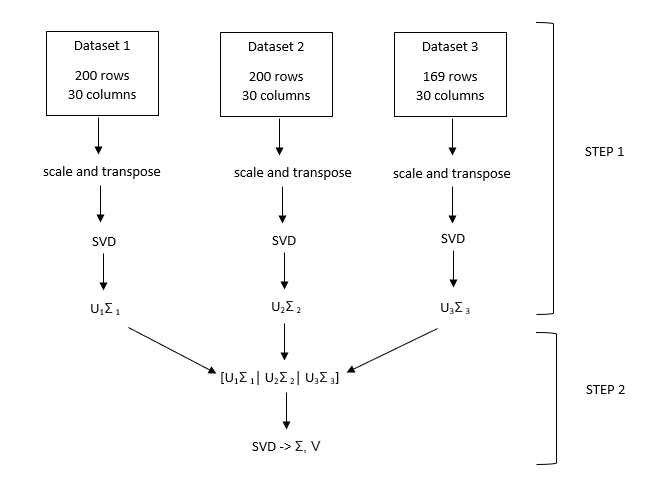
\includegraphics[width=1.5\linewidth]{esquema_exemple1} 

}

\caption{Flowchart of the Block method procedure. The SVD of each of the subdatasets is computed and after that, the results are joined to compute a SVD again. }\label{fig:breast1c}
\end{figure}

To do so, we create a list containing these three datasets and we use
\texttt{getPCA} function. In this case, we do not need to specify the
method because the Block method is by default. It is also important that
the \texttt{getPCA} function has the option to center and scale the
data. By default the function will do it, but we can choose not do so.

\begin{Shaded}
\begin{Highlighting}[]
\NormalTok{data1 <-}\StringTok{ }\NormalTok{num_breast[}\DecValTok{1}\OperatorTok{:}\DecValTok{200}\NormalTok{,]}
\NormalTok{data2 <-}\StringTok{ }\NormalTok{num_breast[}\DecValTok{201}\OperatorTok{:}\DecValTok{400}\NormalTok{,]}
\NormalTok{data3 <-}\StringTok{ }\NormalTok{num_breast[}\DecValTok{401}\OperatorTok{:}\DecValTok{569}\NormalTok{,]}

\NormalTok{data_l <-}\StringTok{ }\KeywordTok{list}\NormalTok{(data1,data2,data3)}

\NormalTok{gpcaL <-}\StringTok{ }\KeywordTok{getPCA}\NormalTok{(data_l)}
\end{Highlighting}
\end{Shaded}

Now we can plot the variables and the individuals again

\begin{Shaded}
\begin{Highlighting}[]

\KeywordTok{par}\NormalTok{(}\DataTypeTok{mfrow=}\KeywordTok{c}\NormalTok{(}\DecValTok{1}\NormalTok{,}\DecValTok{2}\NormalTok{))}
\KeywordTok{plot}\NormalTok{(gpcaL)}
\KeywordTok{plot}\NormalTok{(gpcaL, }\DataTypeTok{type=}\StringTok{"individuals"}\NormalTok{)}
\end{Highlighting}
\end{Shaded}

\begin{figure}

{\centering \includegraphics[width=0.3\linewidth]{svdParallel_files/figure-latex/breast3-1} 

}

\caption{Variables and individuals projections from getPCA function using Block method. Left plot shows the variables into the two first principal components, while right plot corresponds to the individuals.}\label{fig:breast3}
\end{figure}

We can compare the results obtained with function getPCA with other
functions in other R packages. IN the following plots we can see the
results using \texttt{PCA} function in
\href{https://www.rdocumentation.org/packages/FactoMineR}{FactoMineR}
package.

\begin{Shaded}
\begin{Highlighting}[]
\NormalTok{pcaR <-}\StringTok{ }\KeywordTok{PCA}\NormalTok{(num_breast, }\DataTypeTok{graph=}\OtherTok{FALSE}\NormalTok{)}
\KeywordTok{par}\NormalTok{(}\DataTypeTok{mfrow=}\KeywordTok{c}\NormalTok{(}\DecValTok{1}\NormalTok{,}\DecValTok{2}\NormalTok{))}
\KeywordTok{plot}\NormalTok{(pcaR, }\DataTypeTok{choix=}\StringTok{"var"}\NormalTok{, }\DataTypeTok{label=}\StringTok{"none"}\NormalTok{)}
\KeywordTok{plot}\NormalTok{(pcaR, }\DataTypeTok{choix=}\StringTok{"ind"}\NormalTok{, }\DataTypeTok{label=}\StringTok{"none"}\NormalTok{)}
\end{Highlighting}
\end{Shaded}

\begin{figure}

{\centering \includegraphics{svdParallel_files/figure-latex/breast2b-1} 

}

\caption{Variables and individuals projections from PCA function. Left plot shows the variables into the two first principal components, while right plot corresponds to the individuals.}\label{fig:breast2b}
\end{figure}

The results do not match exactly. However, we can appreciate that these
two plots are the two previous ones rotated 180º. This means that they
are the same plots but using the opposite direction of the principal
components. As we know, the principal components are not uniquely
defined as we can take \texttt{u} or \texttt{-u} and they both would be
a principal component. Therefore, the results are coherent.

Now we can also classify them according to the diagnosis of the tumor:
benign or malignant.

\begin{Shaded}
\begin{Highlighting}[]
\NormalTok{m <-}\StringTok{ }\NormalTok{breast[,}\DecValTok{2}\NormalTok{] }\OperatorTok{==}\StringTok{"M"}
\NormalTok{b <-}\StringTok{ }\NormalTok{breast[,}\DecValTok{2}\NormalTok{] }\OperatorTok{==}\StringTok{"B"}
\KeywordTok{plot}\NormalTok{(gpcaL}\OperatorTok{$}\NormalTok{Y[m,}\KeywordTok{c}\NormalTok{(}\DecValTok{1}\NormalTok{,}\DecValTok{2}\NormalTok{)], }\DataTypeTok{main=}\StringTok{"Individuals"}\NormalTok{,}
     \DataTypeTok{type=}\StringTok{"p"}\NormalTok{, }\DataTypeTok{col=}\StringTok{"blue"}\NormalTok{,}\DataTypeTok{xlab=}\StringTok{"PC1 (44.27%)"}\NormalTok{, }\DataTypeTok{ylab=}\StringTok{"PC2(18.97%)"}\NormalTok{, }\DataTypeTok{xlim=}\KeywordTok{c}\NormalTok{(}\OperatorTok{-}\DecValTok{18}\NormalTok{,}\DecValTok{12}\NormalTok{), }\DataTypeTok{ylim=}\KeywordTok{c}\NormalTok{(}\OperatorTok{-}\DecValTok{14}\NormalTok{,}\DecValTok{9}\NormalTok{))}
\KeywordTok{points}\NormalTok{(gpcaL}\OperatorTok{$}\NormalTok{Y[b,}\KeywordTok{c}\NormalTok{(}\DecValTok{1}\NormalTok{,}\DecValTok{2}\NormalTok{)], }\DataTypeTok{col=}\StringTok{"red"}\NormalTok{)}
\KeywordTok{abline}\NormalTok{(}\DataTypeTok{a=}\DecValTok{0}\NormalTok{,}\DataTypeTok{b=}\DecValTok{0}\NormalTok{, }\DataTypeTok{lty=}\DecValTok{3}\NormalTok{)}
\KeywordTok{abline}\NormalTok{(}\DataTypeTok{v=}\DecValTok{0}\NormalTok{, }\DataTypeTok{lty=}\DecValTok{3}\NormalTok{)}
\KeywordTok{legend}\NormalTok{(}\StringTok{"topright"}\NormalTok{, }\DataTypeTok{legend =} \KeywordTok{c}\NormalTok{(}\StringTok{"Malignant"}\NormalTok{, }\StringTok{"Benign"}\NormalTok{), }\DataTypeTok{col=}\KeywordTok{c}\NormalTok{(}\StringTok{"blue"}\NormalTok{, }\StringTok{"red"}\NormalTok{), }\DataTypeTok{pch=}\DecValTok{1}\NormalTok{, }\DataTypeTok{cex=}\FloatTok{0.75}\NormalTok{)}
\end{Highlighting}
\end{Shaded}

\begin{figure}

{\centering \includegraphics{svdParallel_files/figure-latex/breast4-1} 

}

\caption{Principal components of breast dataset. The plot shows the samples according to the group they belong (benign or malignant cancer)}\label{fig:breast4}
\end{figure}

We have been able to compute a PCA of three datasets together without
merging them. This means that this function would be applicable to
DataSHIELD experiments.

\section{Computing a PCA using Block method for omic
data.}\label{computing-a-pca-using-block-method-for-omic-data.}

In this case we will use a larger dataset with omic data. We will use a
\href{https://www.rdocumentation.org/packages/SummarizedExperiment}{SummarizedExperiment}
called \texttt{breastMulti} that contains a
\href{https://www.rdocumentation.org/packages/SummarizedExperiment/versions/1.2.3/topics/RangedSummarizedExperiment-class}{RangeSummarizedExperiment}
called \texttt{breastTCGA}.

\begin{Shaded}
\begin{Highlighting}[]
\NormalTok{breastTCGA <-}\StringTok{ }\NormalTok{breastMulti[[}\StringTok{"expression"}\NormalTok{]]}
\NormalTok{breastTCGA}
\NormalTok{class}\OperatorTok{:}\StringTok{ }\NormalTok{RangedSummarizedExperiment }
\NormalTok{dim}\OperatorTok{:}\StringTok{ }\DecValTok{8362} \DecValTok{79} 
\KeywordTok{metadata}\NormalTok{(}\DecValTok{0}\NormalTok{)}\OperatorTok{:}
\KeywordTok{assays}\NormalTok{(}\DecValTok{1}\NormalTok{)}\OperatorTok{:}\StringTok{ }\NormalTok{genexpr}
\KeywordTok{rownames}\NormalTok{(}\DecValTok{8362}\NormalTok{)}\OperatorTok{:}\StringTok{ }\NormalTok{ABCA6 ABCC12 ... ZNF569 ZNF610}
\NormalTok{rowData }\KeywordTok{names}\NormalTok{(}\DecValTok{0}\NormalTok{)}\OperatorTok{:}
\KeywordTok{colnames}\NormalTok{(}\DecValTok{79}\NormalTok{)}\OperatorTok{:}\StringTok{ }\NormalTok{TCGA}\OperatorTok{-}\NormalTok{C8}\OperatorTok{-}\NormalTok{A12V TCGA}\OperatorTok{-}\NormalTok{A2}\OperatorTok{-}\NormalTok{A0ST ... TCGA}\OperatorTok{-}\NormalTok{B6}\OperatorTok{-}\NormalTok{A0X0}
\NormalTok{  TCGA}\OperatorTok{-}\NormalTok{A2}\OperatorTok{-}\NormalTok{A04Y}
\NormalTok{colData }\KeywordTok{names}\NormalTok{(}\DecValTok{30}\NormalTok{)}\OperatorTok{:}\StringTok{ }\NormalTok{Gender Age.at.Initial.Pathologic.Diagnosis ...}
\NormalTok{  Integrated.Clusters..unsup.exp. id}
\end{Highlighting}
\end{Shaded}

We can extract the dataset containing the genes information using
\texttt{assay} function. There are 8362 variables and 79 individuals.

\begin{Shaded}
\begin{Highlighting}[]
\NormalTok{genes <-}\StringTok{ }\KeywordTok{assay}\NormalTok{(breastTCGA)}
\KeywordTok{dim}\NormalTok{(genes)}
\NormalTok{[}\DecValTok{1}\NormalTok{] }\DecValTok{8362}   \DecValTok{79}
\NormalTok{genes[}\DecValTok{1}\OperatorTok{:}\DecValTok{5}\NormalTok{,}\DecValTok{1}\OperatorTok{:}\DecValTok{12}\NormalTok{]}
\NormalTok{        TCGA}\OperatorTok{-}\NormalTok{C8}\OperatorTok{-}\NormalTok{A12V TCGA}\OperatorTok{-}\NormalTok{A2}\OperatorTok{-}\NormalTok{A0ST TCGA}\OperatorTok{-}\NormalTok{E2}\OperatorTok{-}\NormalTok{A159 TCGA}\OperatorTok{-}\NormalTok{BH}\OperatorTok{-}\NormalTok{A0BW TCGA}\OperatorTok{-}\NormalTok{A2}\OperatorTok{-}\NormalTok{A0SX}
\NormalTok{ABCA6       }\FloatTok{0.804100}     \FloatTok{1.411900}     \FloatTok{0.434300}    \OperatorTok{-}\FloatTok{1.437600}     \FloatTok{0.907800}
\NormalTok{ABCC12     }\OperatorTok{-}\FloatTok{0.653467}    \OperatorTok{-}\FloatTok{0.411000}    \OperatorTok{-}\FloatTok{0.499267}    \OperatorTok{-}\FloatTok{0.939917}    \OperatorTok{-}\FloatTok{0.622000}
\NormalTok{ABCC5       }\FloatTok{0.062833}    \OperatorTok{-}\FloatTok{0.837000}    \OperatorTok{-}\FloatTok{0.531000}    \OperatorTok{-}\FloatTok{0.758667}     \FloatTok{0.034833}
\NormalTok{ABCG8       }\FloatTok{0.125750}    \OperatorTok{-}\FloatTok{0.058250}    \OperatorTok{-}\FloatTok{0.503250}    \OperatorTok{-}\FloatTok{1.636250}     \FloatTok{0.003750}
\NormalTok{ABHD14B    }\OperatorTok{-}\FloatTok{0.915313}    \OperatorTok{-}\FloatTok{0.183188}    \OperatorTok{-}\FloatTok{0.533312}    \OperatorTok{-}\FloatTok{0.846313}    \OperatorTok{-}\FloatTok{0.195687}
\NormalTok{        TCGA}\OperatorTok{-}\NormalTok{AR}\OperatorTok{-}\NormalTok{A1AI TCGA}\OperatorTok{-}\NormalTok{AR}\OperatorTok{-}\NormalTok{A1AQ TCGA}\OperatorTok{-}\NormalTok{A1}\OperatorTok{-}\NormalTok{A0SO TCGA}\OperatorTok{-}\NormalTok{AO}\OperatorTok{-}\NormalTok{A0J6 TCGA}\OperatorTok{-}\NormalTok{BH}\OperatorTok{-}\NormalTok{A0B3}
\NormalTok{ABCA6      }\OperatorTok{-}\FloatTok{0.280100}    \OperatorTok{-}\FloatTok{0.084200}    \OperatorTok{-}\FloatTok{0.893300}    \OperatorTok{-}\FloatTok{1.996800}    \OperatorTok{-}\FloatTok{0.563900}
\NormalTok{ABCC12      }\FloatTok{3.557667}    \OperatorTok{-}\FloatTok{0.359833}    \OperatorTok{-}\FloatTok{0.471167}    \OperatorTok{-}\FloatTok{0.179267}    \OperatorTok{-}\FloatTok{0.758500}
\NormalTok{ABCC5       }\FloatTok{0.731417}    \OperatorTok{-}\FloatTok{1.078000}    \OperatorTok{-}\FloatTok{0.435167}     \FloatTok{0.645667}    \OperatorTok{-}\FloatTok{0.285167}
\NormalTok{ABCG8       }\FloatTok{0.343750}     \FloatTok{0.559750}     \FloatTok{0.240750}    \OperatorTok{-}\FloatTok{0.891750}    \OperatorTok{-}\FloatTok{0.852750}
\NormalTok{ABHD14B    }\OperatorTok{-}\FloatTok{0.816063}    \OperatorTok{-}\FloatTok{0.178312}    \OperatorTok{-}\FloatTok{1.000063}    \OperatorTok{-}\FloatTok{0.383188}    \OperatorTok{-}\FloatTok{0.440437}
\NormalTok{        TCGA}\OperatorTok{-}\NormalTok{C8}\OperatorTok{-}\NormalTok{A134 TCGA}\OperatorTok{-}\NormalTok{A2}\OperatorTok{-}\NormalTok{A0T2}
\NormalTok{ABCA6      }\OperatorTok{-}\FloatTok{0.075100}    \OperatorTok{-}\FloatTok{1.545900}
\NormalTok{ABCC12     }\OperatorTok{-}\FloatTok{0.321333}    \OperatorTok{-}\FloatTok{0.616667}
\NormalTok{ABCC5      }\OperatorTok{-}\FloatTok{0.591000}    \OperatorTok{-}\FloatTok{0.384500}
\NormalTok{ABCG8      }\OperatorTok{-}\FloatTok{0.456750}     \FloatTok{0.088750}
\NormalTok{ABHD14B    }\OperatorTok{-}\FloatTok{0.717438}    \OperatorTok{-}\FloatTok{0.059437}
\end{Highlighting}
\end{Shaded}

As this dataset contains omic data the individuals are in columns and
the variables are in rows. This is not the normal way to build datasets
and our functions require the individuals to be in the rows and the
variables in the columns. This means that we need to apply
\texttt{getPCA} to the transpose of the \texttt{genes} dataset.
Moreover, the Block method has a parameter called \texttt{parts}. This
parameter sets the number of subdatasets to be created from the dataset
under study. The default value is 2. If n is the number of rows and p is
the number of columns of our dataset, this number \texttt{parts} cannot
be greater than max(n,p). We can write to set \texttt{parts=5}.

\begin{Shaded}
\begin{Highlighting}[]
\NormalTok{gpca <-}\StringTok{ }\KeywordTok{getPCA}\NormalTok{(}\KeywordTok{t}\NormalTok{(genes), }\DataTypeTok{parts =} \DecValTok{5}\NormalTok{, }\DataTypeTok{center=}\NormalTok{T, }\DataTypeTok{scale=}\NormalTok{T)}
\KeywordTok{plot}\NormalTok{(gpca, }\DataTypeTok{type=}\StringTok{"individuals"}\NormalTok{)}
\end{Highlighting}
\end{Shaded}

\begin{figure}

{\centering \includegraphics{svdParallel_files/figure-latex/breastTCGA3-1} 

}

\caption{Individuals projections from getPCA function using Block method. The plot shows the individuals into the two first principal components}\label{fig:breastTCGA3}
\end{figure}

In this case we will not plot the variables because there are too many
and the resulting plot is not interpretable.

In the individuals plot we can see two differentiated groups. These
groups correspond to the estrongen status, that can be positive or
negative.

\begin{Shaded}
\begin{Highlighting}[]
\NormalTok{group<-}\KeywordTok{as.factor}\NormalTok{(breastTCGA}\OperatorTok{$}\NormalTok{ER.Status)}
\KeywordTok{plot}\NormalTok{(gpca}\OperatorTok{$}\NormalTok{Y[group}\OperatorTok{==}\StringTok{"Positive"}\NormalTok{,}\KeywordTok{c}\NormalTok{(}\DecValTok{1}\NormalTok{,}\DecValTok{2}\NormalTok{)], }\DataTypeTok{main=}\StringTok{"Individuals"}\NormalTok{,}
       \DataTypeTok{type=}\StringTok{"p"}\NormalTok{, }\DataTypeTok{col=}\StringTok{"blue"}\NormalTok{,}\DataTypeTok{xlab=}\StringTok{"PC1 (17.84%)"}\NormalTok{, }\DataTypeTok{ylab=}\StringTok{"PC2 (7.61%)"}\NormalTok{, }\DataTypeTok{xlim=}\KeywordTok{c}\NormalTok{(}\OperatorTok{-}\DecValTok{60}\NormalTok{,}\DecValTok{70}\NormalTok{), }\DataTypeTok{ylim=}\KeywordTok{c}\NormalTok{(}\OperatorTok{-}\DecValTok{70}\NormalTok{,}\DecValTok{60}\NormalTok{))}
\KeywordTok{points}\NormalTok{(gpca}\OperatorTok{$}\NormalTok{Y[group}\OperatorTok{==}\StringTok{"Negative"}\NormalTok{,}\KeywordTok{c}\NormalTok{(}\DecValTok{1}\NormalTok{,}\DecValTok{2}\NormalTok{)], }\DataTypeTok{col=}\StringTok{"red"}\NormalTok{)}
\KeywordTok{abline}\NormalTok{(}\DataTypeTok{a=}\DecValTok{0}\NormalTok{,}\DataTypeTok{b=}\DecValTok{0}\NormalTok{, }\DataTypeTok{lty=}\DecValTok{3}\NormalTok{)}
\KeywordTok{abline}\NormalTok{(}\DataTypeTok{v=}\DecValTok{0}\NormalTok{, }\DataTypeTok{lty=}\DecValTok{3}\NormalTok{)}
\KeywordTok{legend}\NormalTok{(}\StringTok{"topright"}\NormalTok{, }\DataTypeTok{legend =} \KeywordTok{c}\NormalTok{(}\StringTok{"Positve"}\NormalTok{, }\StringTok{"Negative"}\NormalTok{), }\DataTypeTok{col=}\KeywordTok{c}\NormalTok{(}\StringTok{"blue"}\NormalTok{, }\StringTok{"red"}\NormalTok{), }\DataTypeTok{pch=}\DecValTok{1}\NormalTok{, }\DataTypeTok{cex=}\FloatTok{0.75}\NormalTok{)}
\end{Highlighting}
\end{Shaded}

\begin{figure}

{\centering \includegraphics{svdParallel_files/figure-latex/breastTCGA4-1} 

}

\caption{Principal components of breastTCGA dataset. The plot shows the samples according to their estrongen status.}\label{fig:breastTCGA4}
\end{figure}

There exist specific functions to compute a PCA on gene expression data.
This is the case of function \texttt{ord}. We can see that we obtain
similar results.

\begin{Shaded}
\begin{Highlighting}[]
\NormalTok{group<-}\KeywordTok{as.factor}\NormalTok{(breastTCGA}\OperatorTok{$}\NormalTok{ER.Status)}
\NormalTok{out <-}\StringTok{ }\KeywordTok{ord}\NormalTok{(genes, }\DataTypeTok{classvec=}\NormalTok{group, }\DataTypeTok{type =} \StringTok{"pca"}\NormalTok{)}
\KeywordTok{plot}\NormalTok{(out, }\DataTypeTok{nlab=}\DecValTok{3}\NormalTok{)}
\KeywordTok{plotarrays}\NormalTok{(out)}
\KeywordTok{par}\NormalTok{(}\DataTypeTok{mfrow=}\KeywordTok{c}\NormalTok{(}\DecValTok{1}\NormalTok{,}\DecValTok{1}\NormalTok{))}
\end{Highlighting}
\end{Shaded}

\begin{figure}

{\centering \includegraphics{svdParallel_files/figure-latex/breastTCGA5-1} 

}

\caption{Variables and individuals projections from ord function. First, there is the plot of the eigenvalues. Then, the plot of the variables (top right) and the individuals (bottom left) in the first two principal components, and the individuals classified in groups.}\label{fig:breastTCGA5}
\end{figure}

Apart from method \texttt{blockSVD} there is another method called
\texttt{generalBlockSVD}. This method is the generalization from the
previous one in a multi level algorithm. In order to use it we can set
the parameters \texttt{k} and \texttt{q}. Their default values are 2 and
1, respectively. Parameter \texttt{q} sets the number of levels of the
algorithm (how many times we will repeat the process), and \texttt{k}
sets the number of subdatasets to be concatenated at each level. More
information about the method can be found at (Iwen and Ong 2016).

We can see that the same results can be obtained using this method:

\begin{Shaded}
\begin{Highlighting}[]
\NormalTok{gpca <-}\StringTok{ }\KeywordTok{getPCA}\NormalTok{(}\KeywordTok{t}\NormalTok{(genes),  }\DataTypeTok{method=}\StringTok{"generalBlockSVD"}\NormalTok{, }\DataTypeTok{k=}\DecValTok{2}\NormalTok{, }\DataTypeTok{q=}\DecValTok{2}\NormalTok{)}
\KeywordTok{plot}\NormalTok{(gpca}\OperatorTok{$}\NormalTok{Y[group}\OperatorTok{==}\StringTok{"Positive"}\NormalTok{,}\KeywordTok{c}\NormalTok{(}\DecValTok{1}\NormalTok{,}\DecValTok{2}\NormalTok{)], }\DataTypeTok{main=}\StringTok{"Individuals"}\NormalTok{,}
       \DataTypeTok{type=}\StringTok{"p"}\NormalTok{, }\DataTypeTok{col=}\StringTok{"blue"}\NormalTok{,}\DataTypeTok{xlab=}\StringTok{"PC1 (17.84%)"}\NormalTok{, }\DataTypeTok{ylab=}\StringTok{"PC2 (7.61%)"}\NormalTok{, }\DataTypeTok{xlim=}\KeywordTok{c}\NormalTok{(}\OperatorTok{-}\DecValTok{60}\NormalTok{,}\DecValTok{70}\NormalTok{), }\DataTypeTok{ylim=}\KeywordTok{c}\NormalTok{(}\OperatorTok{-}\DecValTok{70}\NormalTok{,}\DecValTok{60}\NormalTok{))}
\KeywordTok{points}\NormalTok{(gpca}\OperatorTok{$}\NormalTok{Y[group}\OperatorTok{==}\StringTok{"Negative"}\NormalTok{,}\KeywordTok{c}\NormalTok{(}\DecValTok{1}\NormalTok{,}\DecValTok{2}\NormalTok{)], }\DataTypeTok{col=}\StringTok{"red"}\NormalTok{)}
\KeywordTok{abline}\NormalTok{(}\DataTypeTok{a=}\DecValTok{0}\NormalTok{,}\DataTypeTok{b=}\DecValTok{0}\NormalTok{, }\DataTypeTok{lty=}\DecValTok{3}\NormalTok{)}
\KeywordTok{abline}\NormalTok{(}\DataTypeTok{v=}\DecValTok{0}\NormalTok{, }\DataTypeTok{lty=}\DecValTok{3}\NormalTok{)}
\KeywordTok{legend}\NormalTok{(}\StringTok{"topright"}\NormalTok{, }\DataTypeTok{legend =} \KeywordTok{c}\NormalTok{(}\StringTok{"Positve"}\NormalTok{, }\StringTok{"Negative"}\NormalTok{), }\DataTypeTok{col=}\KeywordTok{c}\NormalTok{(}\StringTok{"blue"}\NormalTok{, }\StringTok{"red"}\NormalTok{), }\DataTypeTok{pch=}\DecValTok{1}\NormalTok{, }\DataTypeTok{cex=}\FloatTok{0.75}\NormalTok{)}
\end{Highlighting}
\end{Shaded}

\begin{figure}

{\centering \includegraphics{svdParallel_files/figure-latex/breastTCGA6-1} 

}

\caption{Individuals projections from getPCA function using General Block method. The plot shows the individuals into the two first principal components classified according to their estrongen status.}\label{fig:breastTCGA6}
\end{figure}

Finally we can compare the different functions performance using the
function \texttt{microbenchmark}. It computes the computation time of
the functions and returns a table with the results.

\begin{Shaded}
\begin{Highlighting}[]
\NormalTok{mb <-}\StringTok{ }\NormalTok{microbenchmark}\OperatorTok{::}\KeywordTok{microbenchmark}\NormalTok{(}\StringTok{"Block method (k=2)"}\NormalTok{=}\KeywordTok{getPCA}\NormalTok{(}\KeywordTok{t}\NormalTok{(genes), }\DataTypeTok{parts =} \DecValTok{2}\NormalTok{, }\DataTypeTok{center=}\NormalTok{F, }\DataTypeTok{scale=}\NormalTok{F),}
                               \StringTok{"Block method (k=5)"}\NormalTok{=}\KeywordTok{getPCA}\NormalTok{(}\KeywordTok{t}\NormalTok{(genes), }\DataTypeTok{parts =} \DecValTok{5}\NormalTok{, }\DataTypeTok{center=}\NormalTok{F, }\DataTypeTok{scale=}\NormalTok{F),}
                               \StringTok{"General Block method (k=2, q=2)"}\NormalTok{=}\KeywordTok{getPCA}\NormalTok{(}\KeywordTok{t}\NormalTok{(genes), }\DataTypeTok{method=}\StringTok{"generalBlockSVD"}\NormalTok{, }\DataTypeTok{k=}\DecValTok{2}\NormalTok{, }\DataTypeTok{q=}\DecValTok{2}\NormalTok{, }\DataTypeTok{center=}\NormalTok{F, }\DataTypeTok{scale=}\NormalTok{F),}
                               \StringTok{"General Block method (k=3, q=2)"}\NormalTok{=}\KeywordTok{getPCA}\NormalTok{(}\KeywordTok{t}\NormalTok{(genes), }\DataTypeTok{method=}\StringTok{"generalBlockSVD"}\NormalTok{, }\DataTypeTok{k=}\DecValTok{3}\NormalTok{, }\DataTypeTok{q=}\DecValTok{2}\NormalTok{, }\DataTypeTok{center=}\NormalTok{F, }\DataTypeTok{scale=}\NormalTok{F),}
                               \StringTok{"PCA function"}\NormalTok{=}\KeywordTok{PCA}\NormalTok{(}\KeywordTok{t}\NormalTok{(genes), }\DataTypeTok{graph=}\OtherTok{FALSE}\NormalTok{), }
                               \StringTok{"ord function"}\NormalTok{ =}\StringTok{ }\KeywordTok{ord}\NormalTok{(genes, }\DataTypeTok{classvec=}\NormalTok{group, }\DataTypeTok{type =} \StringTok{"pca"}\NormalTok{), }\DataTypeTok{times=}\DecValTok{10}\NormalTok{)}
\NormalTok{ggplot2}\OperatorTok{::}\KeywordTok{autoplot}\NormalTok{(mb)}
\end{Highlighting}
\end{Shaded}

\begin{figure}

{\centering \includegraphics{svdParallel_files/figure-latex/breastTCGA7-1} 

}

\caption{Violinplot of the computational times for different functions. The two in the bottom are done using Block method and the following two are using General Block method. The second has been done using PCA function and the first one is using ord function.}\label{fig:breastTCGA7}
\end{figure}

If we look at the mean column we can see that the \texttt{PCA} function
is the one that last more in average. This can be explained because this
function computes a lot of different values a part from the necessary
ones to compute a basic PCA. This also happens with function
\texttt{ord}. These functions compute other scores and it makes it
difficult to compare them with the others. The best way to analyze our
functions' performance is to compare it to the function
\texttt{getPCA0}. This function computes a basic PCA using only one SVD
of the whole matrix. Our \texttt{getPCA} functions are faster in this
case than \texttt{PCA} and \texttt{ord}, but it does not necessarily
mean that they are more efficient.

\begin{Shaded}
\begin{Highlighting}[]
\NormalTok{mb2 <-}\StringTok{ }\NormalTok{microbenchmark}\OperatorTok{::}\KeywordTok{microbenchmark}\NormalTok{(}\StringTok{"Block method (k=2)"}\NormalTok{=}\KeywordTok{getPCA}\NormalTok{(}\KeywordTok{t}\NormalTok{(genes), }\DataTypeTok{parts =} \DecValTok{2}\NormalTok{, }\DataTypeTok{center=}\NormalTok{F, }\DataTypeTok{scale=}\NormalTok{F),}
                               \StringTok{"Block method (k=5)"}\NormalTok{=}\KeywordTok{getPCA}\NormalTok{(}\KeywordTok{t}\NormalTok{(genes), }\DataTypeTok{parts =} \DecValTok{5}\NormalTok{, }\DataTypeTok{center=}\NormalTok{F, }\DataTypeTok{scale=}\NormalTok{F),}
                               \StringTok{"General Block method (k=2, q=2)"}\NormalTok{=}\KeywordTok{getPCA}\NormalTok{(}\KeywordTok{t}\NormalTok{(genes), }\DataTypeTok{method=}\StringTok{"generalBlockSVD"}\NormalTok{, }\DataTypeTok{k=}\DecValTok{2}\NormalTok{, }\DataTypeTok{q=}\DecValTok{2}\NormalTok{, }\DataTypeTok{center=}\NormalTok{F, }\DataTypeTok{scale=}\NormalTok{F),}
                               \StringTok{"General Block method (k=3, q=2)"}\NormalTok{=}\KeywordTok{getPCA}\NormalTok{(}\KeywordTok{t}\NormalTok{(genes), }\DataTypeTok{method=}\StringTok{"generalBlockSVD"}\NormalTok{, }\DataTypeTok{k=}\DecValTok{3}\NormalTok{, }\DataTypeTok{q=}\DecValTok{2}\NormalTok{, }\DataTypeTok{center=}\NormalTok{F, }\DataTypeTok{scale=}\NormalTok{F),}
                               \StringTok{"PCA0 no method"}\NormalTok{=}\KeywordTok{getPCA0}\NormalTok{(}\KeywordTok{t}\NormalTok{(genes), }\DataTypeTok{center=}\NormalTok{F, }\DataTypeTok{scale=}\NormalTok{F),  }\DataTypeTok{times=}\DecValTok{10}\NormalTok{)}

\NormalTok{ggplot2}\OperatorTok{::}\KeywordTok{autoplot}\NormalTok{(mb2)}
\end{Highlighting}
\end{Shaded}

\begin{figure}

{\centering \includegraphics{svdParallel_files/figure-latex/breastTCGA8-1} 

}

\caption{Violinplot of the computational times for different functions. The two in the bottom are done using Block method and the following two have been done using General Block method. The one in the top is using PCA0, it does not use any method.}\label{fig:breastTCGA8}
\end{figure}

The size of the \texttt{genes} dataset is not very big so the
differences between the different functions are not significant. The
performance of the Block method gets better when the size of the dataset
increases.

When the size of the dataset is really large, we should use the parallel
version of the two methods: \texttt{parBlockSVD} and
\texttt{parGeneralBlockSVD}. They work as \texttt{blockSVD} and
\texttt{generalBlokSVD}, respectively.

\section*{References}\label{references}
\addcontentsline{toc}{section}{References}

\hypertarget{refs}{}
\hypertarget{ref-ref}{}
Iwen, Mark, and Benjamin Ong. 2016. ``A Distributed and Incremental Svd
Algorithm for Agglomerative Data Analysis on Large Networks.''


\end{document}
